\newpage
\section{Angabe}
    Implementieren Sie Quicksort (https://de.wikipedia.org/wiki/Quicksort) für arrays mit integern. Testen und Messen sie die Zeiten mit 10, 100, 1000, 10000, 100000 Elementen.

    Bonus Aufgabe: Messreihe und Vergleich mit Bubblesort, messen gegen qsort(3) aus der C Bibliothek.

    \begin{lstlisting}[language=C, style=CStyle, caption=init-CLOCK, captionpos=b, label=init-CLOCK]
#include <assert.h>
#include <stdio.h>
#include <stdlib.h>
#include <time.h>

void qs(int *a, int us, int os)
{
	// TODO
}

// creates a array of size size and fills it with random ints in range 0 to max_int
int *create_array(int size, int max_int)
{
	int *b = (int*)malloc(size * sizeof(int));

	for (int i=0; i<size; i++) {
		b[i] = rand() % max_int;
	}

	return b;
}

#define MY_SIZE 32

int main(int argc, char **argv)
{
	// create random ints based in current time
	srand(time(NULL));

        int *a = create_array(MY_SIZE, 100);

	qs(a, 0, MY_SIZE);

	int old = -1;
	for (int i=0; i<MY_SIZE; ++i)      {
		if (old != -1) assert(old <= a[i]);
		printf("%d ", a[i]);
		old = a[i];
	}
	printf("\n");
}
        \end{lstlisting}

\section{Lösung}
    Die Lösung für den QSort Algorithmus wurde mithilfe des Pseudocodes des wikipedia Artikels \url{https://de.wikipedia.org/wiki/Quicksort} erstellt.\\
    Bublesort wurde aus einem alten Projekt herausgenommen.\\   
    \textbf{Der Code mit Makefile ist in dem extra Zip Ordner oder auf GitHub zu finden: \url{https://github.com/FabioPlunser/FSST_Lezuo/tree/main/Programme/Sortieren}}
\section{Ergebnisse}
    Alle Ergebnisse wurden mit der entsprechenden Größe des Arrays und dies 100mal sortiert, für quasi 100 Messpunkte.
    Ebenfalls erhört sich die höchste Zahl im Array proportional zur größe des Arrays, somit ist bei einer Array Größe von 1000 die höchste
    Zahl auch 1000.
    
    \begin{figure}[!htb]
        \centering
        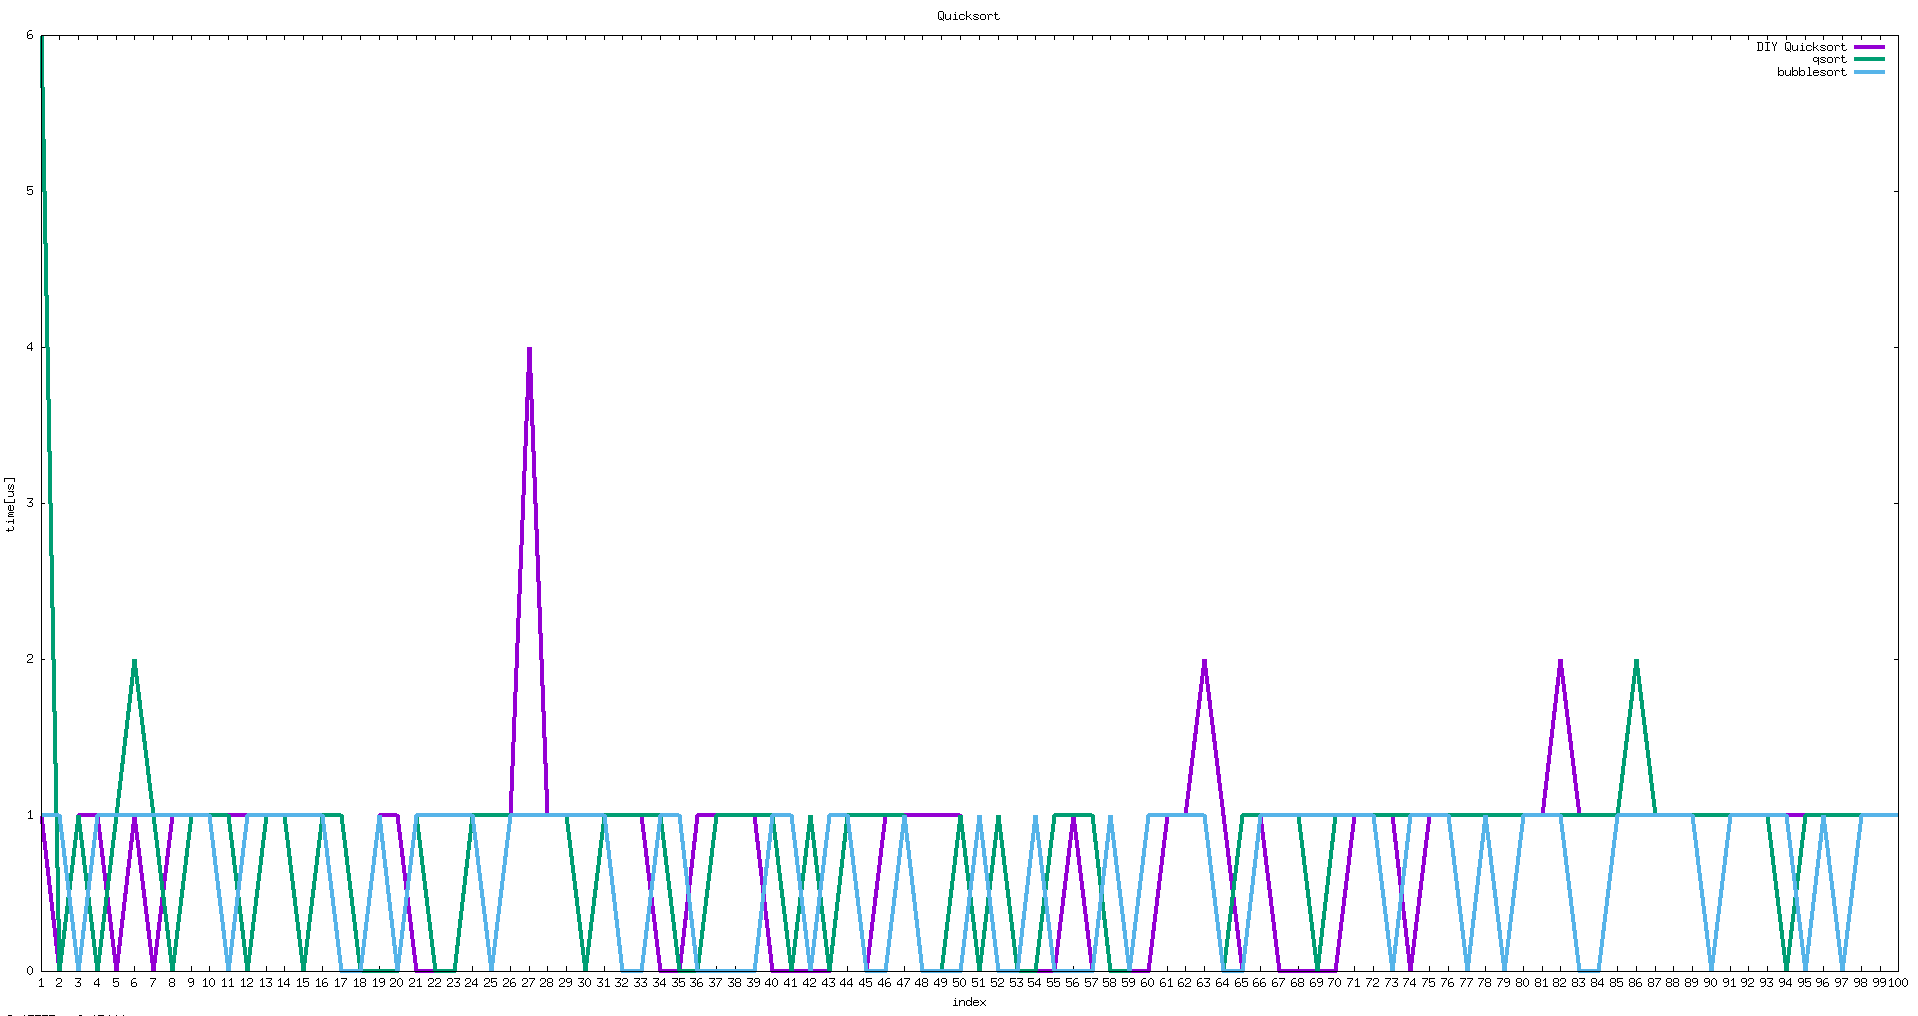
\includegraphics[width=\linewidth]{Sortieren-10.png}
        \caption{Sortieren-10}
        \label{caption:Sortieren-10}
    \end{figure}
    
\newpage
    \begin{figure}[!htb]
        \centering
        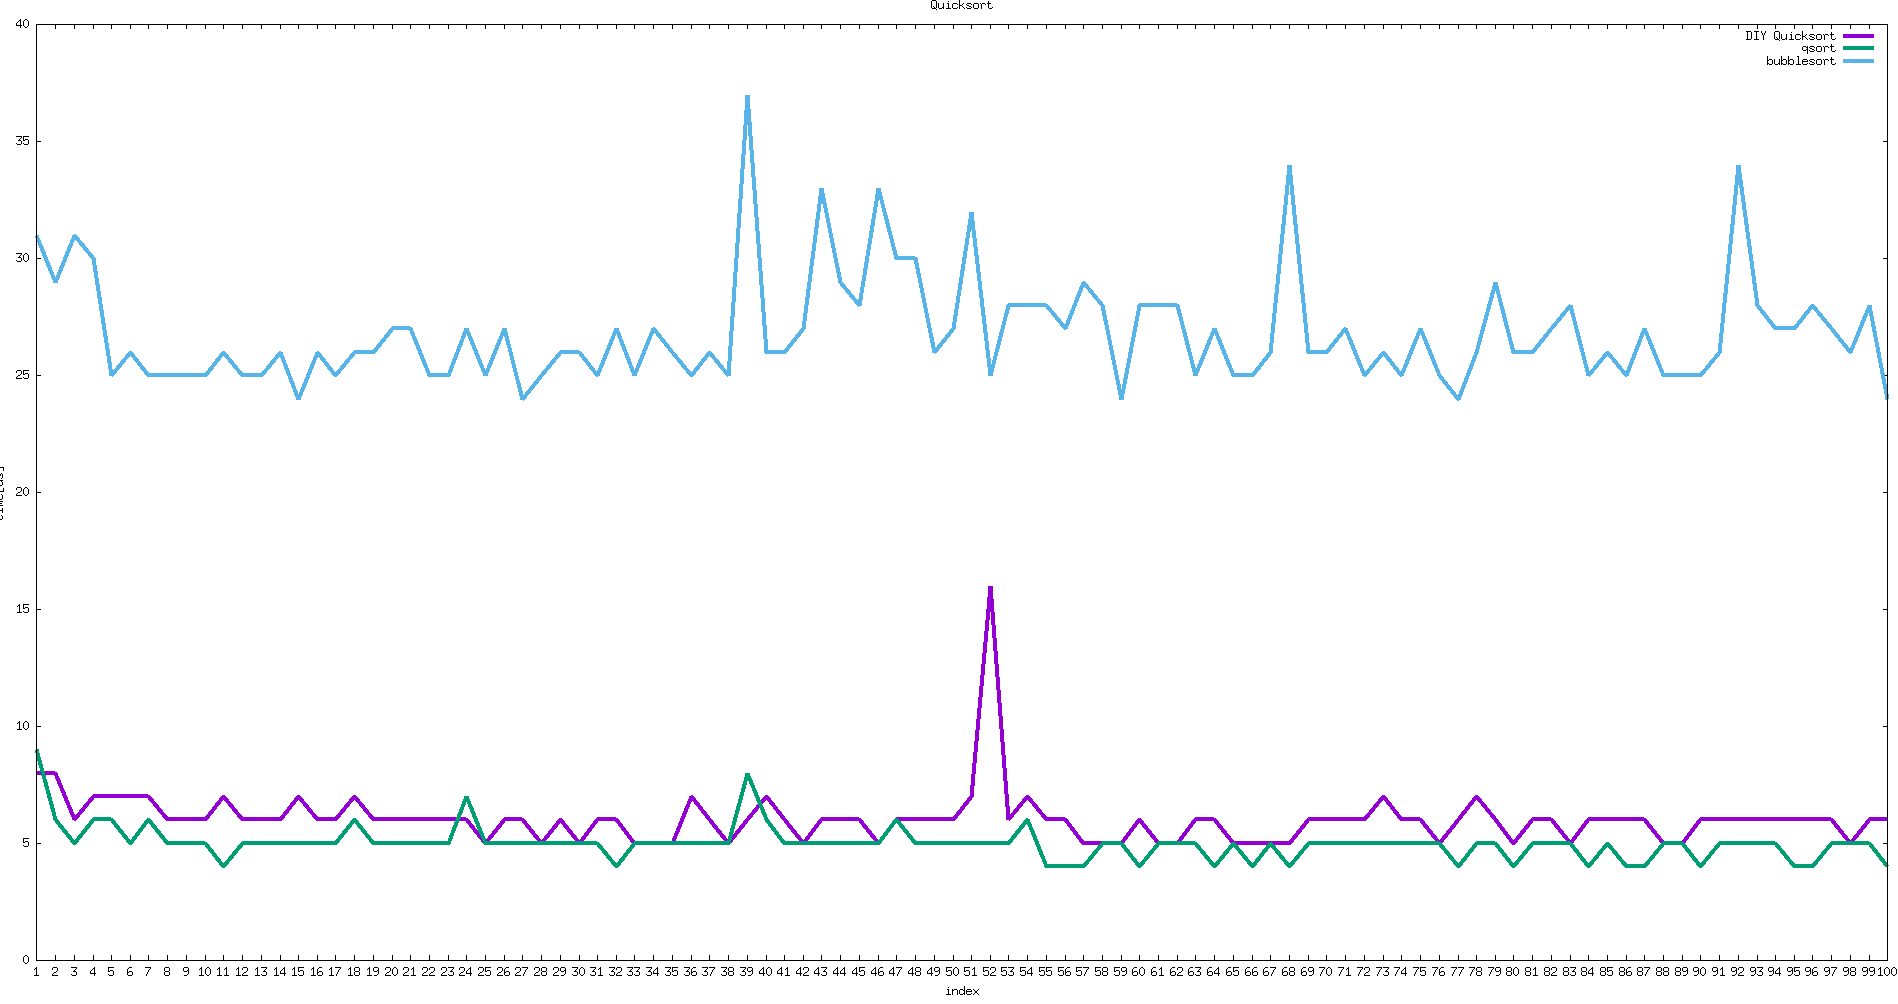
\includegraphics[width=\linewidth]{Sortieren-100.png}
        \caption{Sortieren-100}
        \label{caption:Sortieren-100}
    \end{figure}
    
    \begin{figure}[!htb]
        \centering
        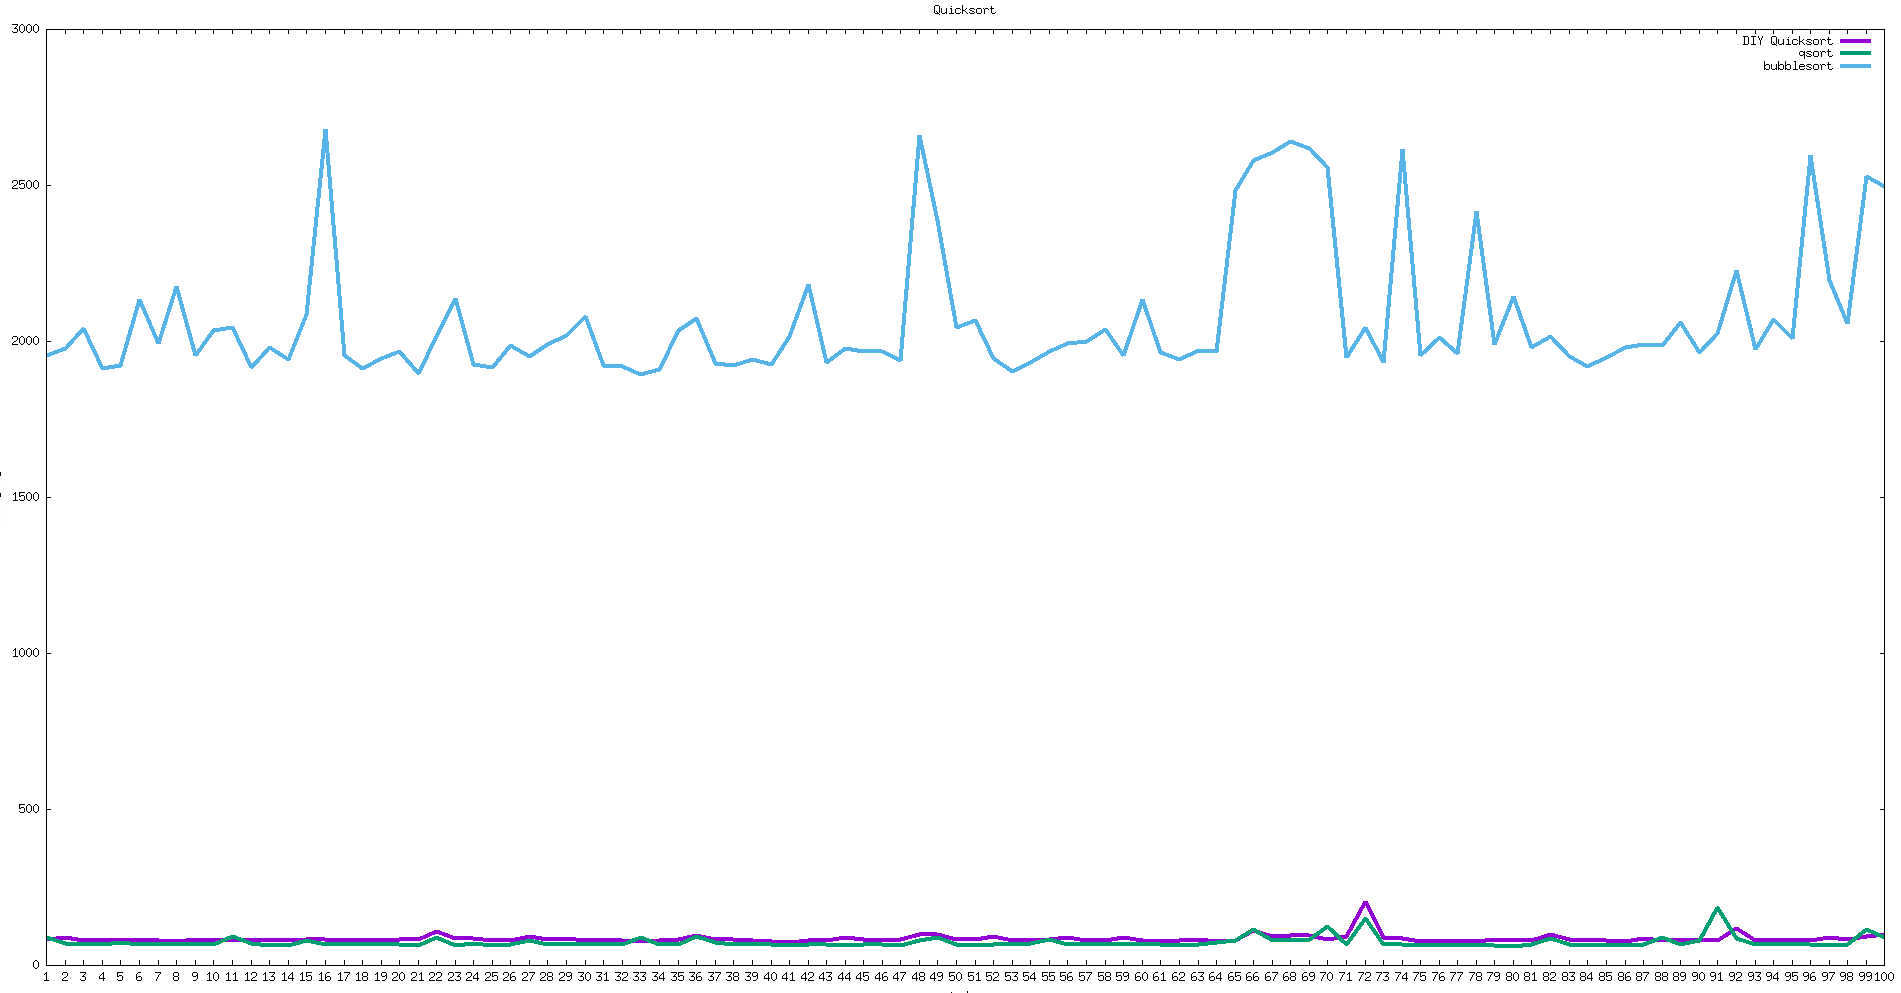
\includegraphics[width=\linewidth]{Sortieren-1000.png}
        \caption{Sortieren-1000}
        \label{caption:Sortieren-1000}
    \end{figure}
    
\newpage
    \begin{figure}[!htb]
        \centering
        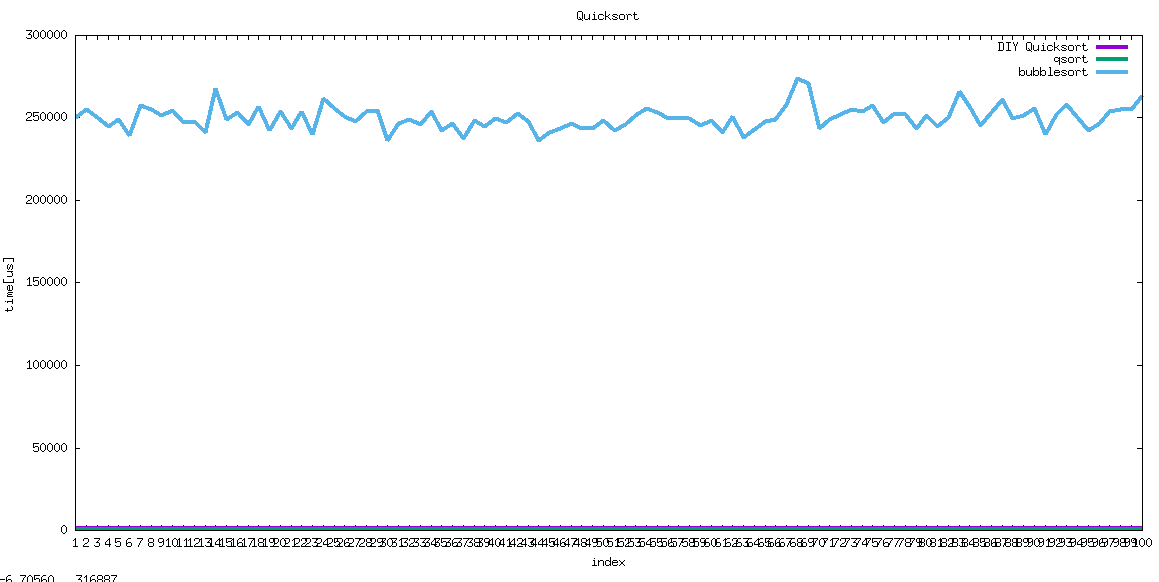
\includegraphics[width=\linewidth]{Sortieren-10000.png}
        \caption{Sortieren-10000}
        \label{caption:Sortieren-10000}
    \end{figure}
    
    \begin{figure}[!htb]
        \centering
        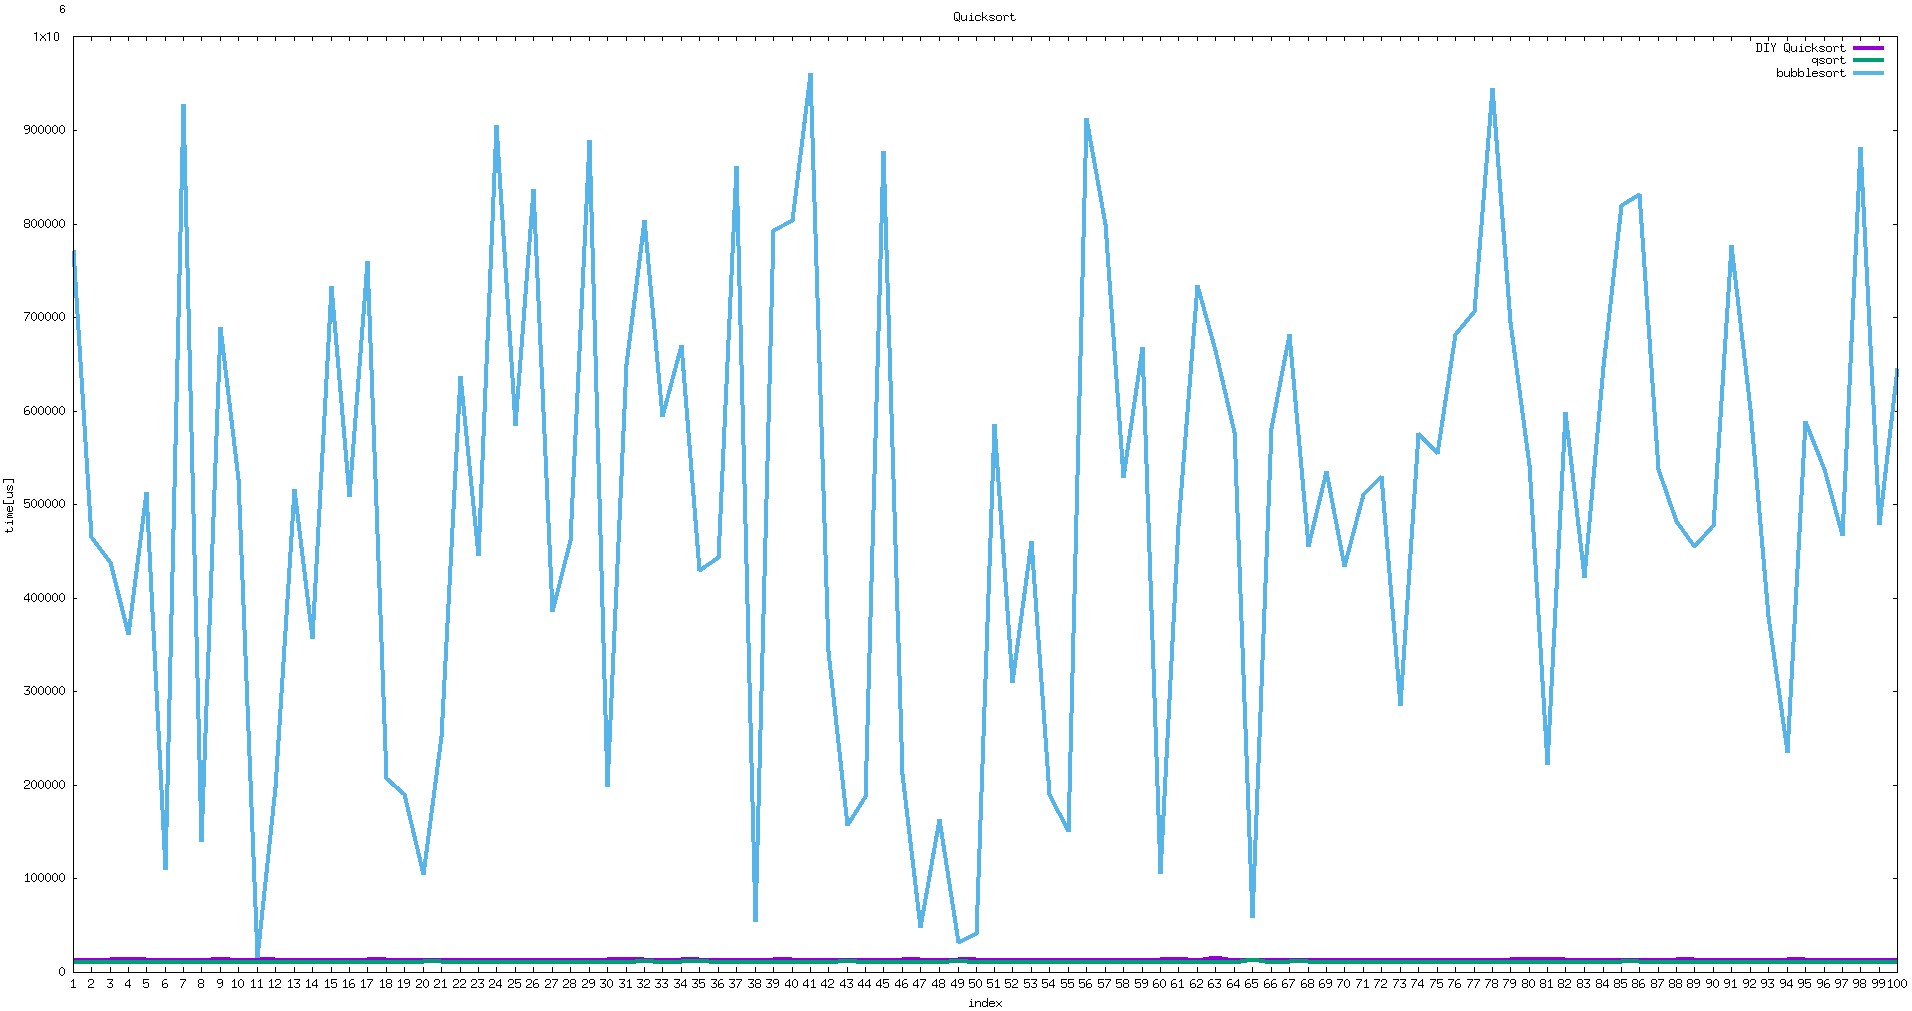
\includegraphics[width=\linewidth]{Sortieren-100000.png}
        \caption{Sortieren-100000}
        \label{caption:Sortieren-100000}
    \end{figure}
    
\newpage
    \noindent Man sieht, das BubleSort immer langsamer wird bei einer Array Größe von 1000 Zahlenwerten benötigt es schon ca. $2500\mu s = 0,0025s$\\
    Bei einer Anzahl von 10000 Werten sind es schon $250000\mu s = 0,25$. Das sind über 4 Minuten.\\
    Bei einer Array Größe von 100000 schwank BubleSort sehr stark von einmal gleich schnell wie QSort bis zu $900000\mu s = 0,9$.